\newif\ifpagetuning

\pagetuningtrue % trying to get page breaks in the best spots

\newif\ifnotcutting \notcuttingfalse % set if not cutting down to size

\newif\iffinaldraft \finaldrafttrue % true if it's the final version


 \newif\ifpdfmadness

\ifx\pdfoutput\undefined
   \pdfmadnessfalse
\else
   \ifnum\pdfoutput=1
     \pdfmadnesstrue
   \else
     \pdfmadnessfalse
   \fi
\fi

\documentclass[nonatbib,preprint,blockstyle,times]{sigplanconf}
  % at 9pt anything but block style is unreadable

\newcommand\mrfy{MRFy} % damn you Noah

\newcommand\txprobj[3][]{a#1_{#2_{j-1}#3_j}}
\newcommand\txprobjj[3][]{a#1_{#2_{j-1}#3_j}}
\newcommand\alignwidth{\ensuremath C} % number of columns in an alignment
\newcommand\pairedwith[1]{{\pi(#1)}}

\ifpagetuning
  \newcommand\tuningbox{\vbox}
\else
  \newcomming\tuningbox{\relax}
\fi

\newcommand\naive{na\"\i ve}
\usepackage{url}
\usepackage{amsmath}
\usepackage{array}
\usepackage{listings}
\usepackage{graphicx}
\lstset{
    tabsize = 2,
    basicstyle = \ttfamily,
    language = Haskell
    }    

\newcommand\figref[1]{Figure~\ref{#1}}
\newcommand\secref[1]{Section~\ref{sec:#1}}
\newcommand\seclabel[1]{\label{sec:#1}}

\usepackage{verbatim}

\newif\ifverbatimsmall
\verbatimsmallfalse
\makeatletter
\def\verbatim@font{%
   \normalfont\ttfamily
   \ifverbatimsmall\small\fi
   \hyphenchar\font\m@ne
   \@noligs}
\makeatother

\newenvironment{smallverbatim}{\par\small\verbatimsmalltrue\verbatim}{\endverbatim}
\newcommand\smallverbatiminput[1]{%
  \everypar=\expandafter{\the\everypar
       \verbatimsmallfalse
%       \belowdisplayskip=\abovedisplayskip
%       \belowdisplayshortskip=\abovedisplayshortskip
       \topsep=\standardvspace}%
  \topsep=0.78\topsep
%  \belowdisplayskip=0.78\belowdisplayskip
%  \belowdisplayshortskip=0.78\belowdisplayshortskip
  \verbatimsmalltrue\verbatiminput{#1}}
\newcommand\smallverbatiminputx[1]{\vspace*{-8pt}{\small\verbatiminput{#1}}} % WTF?? {\LaTeX} hell
\newcommand\smallfuzzverbatiminput[2]{{\par\unskip\small\hfuzz=#1 \verbatiminput{#2}}}

\renewcommand\ttdefault{aett}

  \long\def\remark#1{%
      \ifvmode
         \marginpar{\raggedright\hbadness=10000
         \parindent=8pt \parskip=2pt
         \def\baselinestretch{0.8}\tiny
         \itshape\noindent #1\par}%
      \else
          \unskip\raisebox{-3.5pt}{\rlap{$\scriptstyle\diamond$}}%
          \marginpar{\raggedright\hbadness=10000
         \parindent=8pt \parskip=2pt
         \def\baselinestretch{0.8}\tiny
         \itshape\noindent #1\par}%
      \fi}

\iffinaldraft
  \newcommand\finalremark{\remark}
\else
  \newcommand\finalremark[1]{\relax}
\fi

\usepackage[authoryear]{natbib}
\bibpunct();A{},
\let\cite\citep
\let\citeyearnopar=\citeyear
\let\citeyear=\citeyearpar


\begin{document}
\parskip=0.9\parskip % cheating


\conferenceinfo{ICFP'12,} {September 9--15, 2012, Copenhagen, Denmark.}
\CopyrightYear{2012}
\copyrightdata{978-1-4503-1054-3/12/09}

%\titlebanner{banner above paper title}        % These are ignored unless
\preprintfooter{Haskell in Computational Biology}   % 'preprint' option specified.

\title{Experience Report: Haskell in Computational Biology}
% \subtitle{Subtitle Text, if any}


\authorinfo{Noah M. Daniels \and Andrew Gallant \and Norman Ramsey}
           {Department of Computer Science, Tufts University}
           {{\rmfamily\{}ndaniels, agallant, nr{\rmfamily\}}@cs.tufts.edu}


\maketitle

%
% It can't hurt to remind everyone involved exactly what an Experience
% Report is.
%
%
\begin{abstract}
%An Experience Report provides {evidence} that functional
%programming really works, or it describes obstacles that prevent
%functional programming from working.   
Haskell gives computational biologists
the flexibility and rapid prototyping of a scripting
language but performance comparable to~C++.
In~our experience, higher-order functions, lazy evaluation, and
monads really worked, but
profiling and debugging presented obstacles.
Haskell libraries vary greatly:
memoization combinators and parallel-evaluation
strategies helped us a lot,
but other, nameless libraries mostly got in our way.
Despite the obstacles and the uncertain quality of some libraries,
Haskell's ecosystem
made it easy for us to develop new algorithms in computational
biology.
\end{abstract}

\category{J.3}{Biology and genetics}{}
\category{D.3.2}{Language Classifications}{Applicative (functional) languages}
% \category{CR-number}{subcategory}{third-level}
% 
% \terms
% term1, term2
% 
% \keywords
% keyword1, keyword2

\section{Introduction}

Computational biologists write software that answers questions about 
sequences of nucleic acids (genomic data) or sequences of amino 
acids (proteomic data). 
When performance is paramount,
software is usually written in C~or~C++. 
When convenience, readability, and
productivity are more important,
software is usually written in a dynamically typed
or domain-specific language like
Perl, Python, Ruby, SPSS, or~R.
In~this paper, we report on experience using a third kind of language,
Haskell: 
\begin{itemize}
\item
We had to reimplement an
algorithm already implemented in~C++, 
and the Haskell code is slower.
But the implementation required little effort;
the connection between code and
algorithm is unusually clear (\secref{viterbi});
the code was easy to parallelize; 
and it meets our performance needs
(\secref{perf}).
Moreover, measured as a whole, the software that incorporates this new
code 
performs significantly
better than the~C++ software that preceded~it.
\item
Higher-order functions made it unusually easy to
create and experiment with new stochastic-search algorithms
(\secref{hofs}).
\item
Haskell slowed us down in only one area:  understanding and
improving
performance (\secref{awkward-profiling}).
%%  \item
%%  The only significant impediment that Haskell presented to our
%%  research was the difficulty of understanding and improving the
%%  performance of Haskell programs (\secref{awkward-profiling}).
\item
Although the first two authors are computational
biologists with little background in functional programming,
we~used Haskell successfully.
And Haskell has made it easy to explore new research ideas;
by~contrast,
our group's C++ code has not been a good vehicle for exploring new ideas
(\secref{comparo}).
\item
The Haskell community offers libraries and tools that
promise powerful abstractions.
Some worked as advertised, saved us lots of effort, and were a pleasure
to~use.
Others, not so much.
And~we could not tell ahead of time which experience we were likely to have
 (\secref{penumbra}).
\end{itemize}




\section{The biology}

Proteins %%% are cellular machinery. They
interact with one another and with other 
molecules to carry out the functions of living cells: metabolism, regulation, 
signaling, and so on.
A~protein's function is determined by its structure, 
and its structure is determined by the sequence of amino acids that
form the protein.
The amino-acid sequence is ultimately determined by a sequence of
nucleic acids in DNA, which we call a gene.
Given a genetic sequence, biologists wish to know the cellular
function of the protein that gene codes for.
One of the best known methods of discovering such function is
to find other proteins of 
similar structure, which likely share similar function.
Proteins that share structure and function are expected to be
descended from a common ancestor---in biological terms, \emph{homologous}---and
thus
the problem of identifying proteins similar to a \textit{query sequence} is called 
\textit{homology detection}.




Computational biologists detect homologies by building 
algorithms which, given a {query sequence}, %% of amino acids,
find known proteins of similar structure.
When similar proteins are formed from amino-acid sequences that
are not too different from the query sequence, the homology can be
detected by
a family of algorithms called 
\textit{hidden Markov models}~\cite{Eddy:1998ut}.
But in real biological systems,
proteins with similar structure and function may be formed from significantly 
different amino-acid sequences, which are not close in edit distance.
Our~research software, MRFy (pronounced
``Murphy''), can detect homologies 
in amino-acid sequences that are only distantly related.
%
%We will explain an 
%algorithm for detecting reasonably similar sequences, and then move on to 
%explain MRFy, our novel approach for detecting more distantly related sequences 
%for proteins that share similar structure and function.
%

%
% I hope the new intro renders these two sentences unnecessary. ---NR
%
%
%%  
%%  To~enable you to understand our experience with Haskell,
%%  we~sketch not only the MRFy algorithm (\secref{mrfy})
%%  but also one of the older hidden-Markov algorithms (\secref{viterbi}),
%%  which is incorporated into~MRFy.


\section{The software}



Homology-detection software is most often used in one of two ways:
to test a hypothesis about 
the function of a single, newly discovered protein, or 
to compare every protein in a genome against a library of known protein 
structures.
Either way, 
the software is \emph{trained}
on a group of proteins that share function and structure.
These proteins are identified by a biologist, who puts
their amino-acid sequences into an
\emph{alignment}. 
This alignment relates individual amino acids in a set of homologous proteins.
An~alignment may be represented as a matrix
in which each row corresponds to the amino-acid sequence of a protein,
and each column groups amino acids that play similar roles in
different proteins (Figure~\ref{alignment}).


An alignment may contain \emph{gaps}, which in 
\figref{alignment} are shown as dashes.
A~gap in row~2, column~$j$ indicates that as proteins evolved, either 
protein~2 lost its amino acid in position~$j$, or 
other proteins gained an amino acid in position~$j$.
If~column~$j$ contains few gaps, 
it~is considered a \emph{consensus column},
and the few proteins with gaps probably lost amino acids via
\emph{deletions}.
%%  \remark{NMD: Missing is the fact that all these models
%%  are directionless; they don't care whether something was gained or lost
%%  over time. But this doesn't matter.}
If~column~$j$ contains \emph{mostly} gaps, 
it~is considered a \emph{non-consensus column},
and the few proteins without gaps probably gained amino acids via
\emph{insertions}. 

Once a protein alignment is constructed, it~is used to train a
\emph{hidden Markov model}. 
A~hidden Markov model is a probabilistic finite-state machine which 
can assign a probability to any query sequence.
A~protein whose query sequence has a higher probability is more likely to %
be homologous to the proteins in the alignment.
We~write a query sequence as $x_1, \ldots, x_{\scriptscriptstyle N}$,
where each $x_i$~is 
an amino acid.
$N$~need not be the same as the number of columns in the alignment,
which we write~\alignwidth.


\begin{figure}
\ifpdfmadness
\centerline{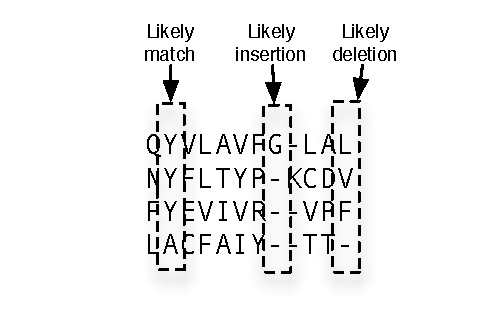
\includegraphics[width=6cm]{alignment.pdf}} 
\else
\centerline{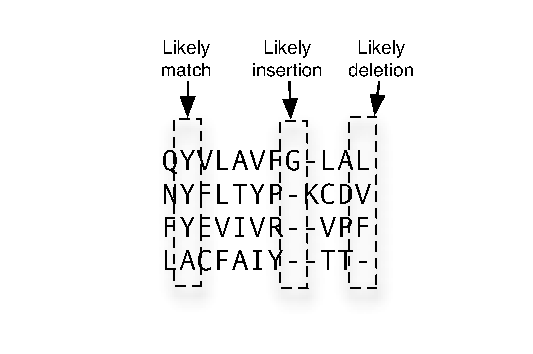
\includegraphics[width=6cm]{alignment.eps}} 
\fi

\caption{A~structural alignment of four proteins $(\alignwidth = 12)$}
\label{alignment} 
\end{figure}



A~hidden Markov model carries probabilities on some states and on all
state transitions.
Both the probabilities and the states are determined by the alignment:
\remark{These bullets need proper parallel structure}
\begin{itemize}
\item
For each column~$j$ of the alignment, the hidden Markov model has a
\emph{match state}~$M_j$.
The match state contains a table $e_{M_j}(x)$ which gives the
 probability that a homologous protein has amino acid~$x$ in
 column~$j$.
This probability is called an \emph{emission} probability.
\item 
For each column~$j$ of the alignment, the hidden Markov model has an
\emph{insertion state}~$I_j$.
The insertion state contains a table $e_{I_j}(x)$ which gives the
probability that a homologous protein has gained amino acid~$x$ by
insertion at column~$j$.
\item
For each column~$j$ of the alignment, the hidden Markov model has a
\emph{deletion state}~$D_j$.
The deletion state determines the probability that the query sequence
has \emph{no} amino acid  in column~$j$, i.e., that it has a gap.
\end{itemize}
The hidden Markov model also has distinguished \emph{begin} and \emph{end} states.
In~our representation, each state contains a probability or a table of
probabilities, and it is also labelled with one of these labels:
\smallverbatiminput{statelabel}


We~use the ``Plan7'' hidden Markov model, which forbids direct
transitions between insertion 
states and deletion states \cite{Eddy:1998ut}. 
The model gets its name because there are exactly
seven possible transitions
into the states of any column~$j$.
Each transition has its own probability:
\remark{Norman: how do you propose to make the subscripts more readable?}
\begin{itemize} 
\item
A~transition into a match state 
is more likely when column~$j$ is a consensus column.
Depending on the predecessor state, 
the probability of such a transition is 
$\txprobj M M$, $\txprobj I M$, or~$\txprobj D M$.
\item
A~transition into a deletion state 
is more likely when column~$j$ is a non-consensus column.
The probability of such a transition is 
$\txprobj M D$~or~$\txprobj D D$.
\item
A~transition into an insertion state 
is more likely when column~$j$ is a non-consensus column.
The probability of such a transition is 
$\txprobjj M I$~or~$\txprobjj I I$.
\end{itemize}



\begin{figure} 
\ifpdfmadness
\centerline{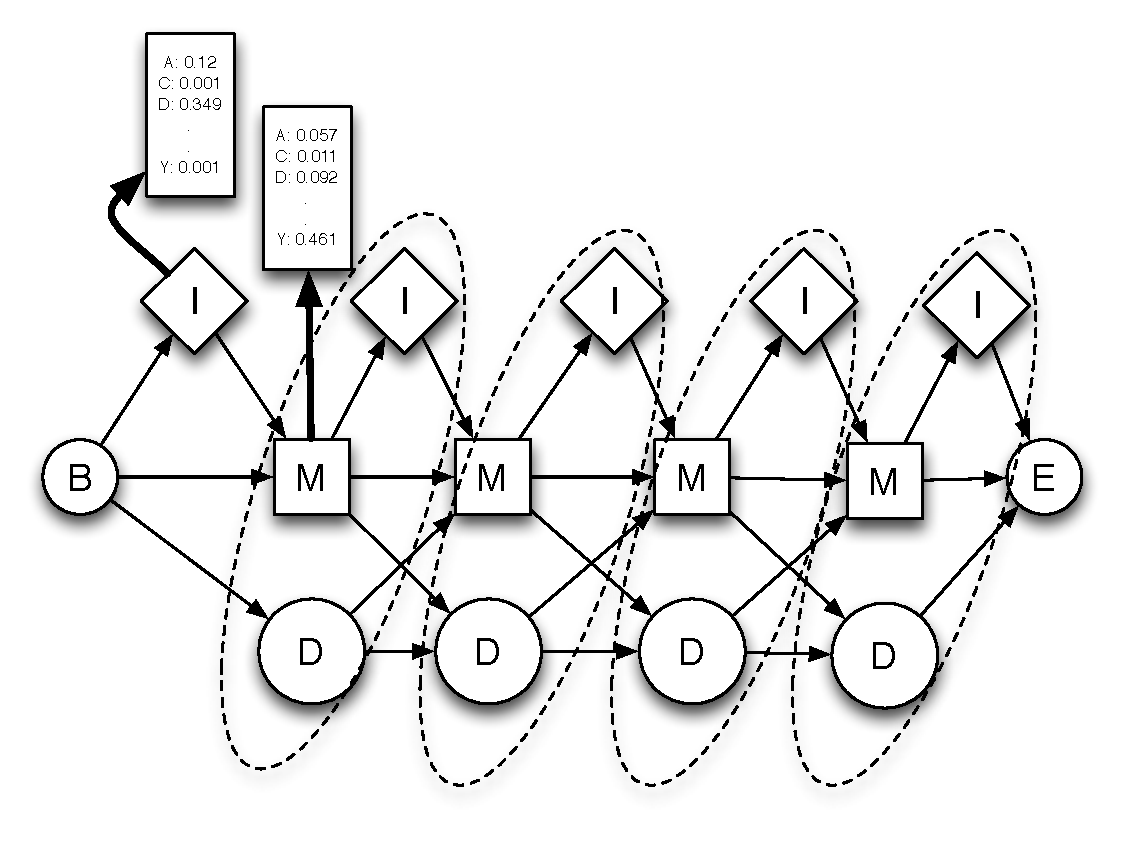
\includegraphics[width=8cm]{Plan7.pdf}} 
\else
\centerline{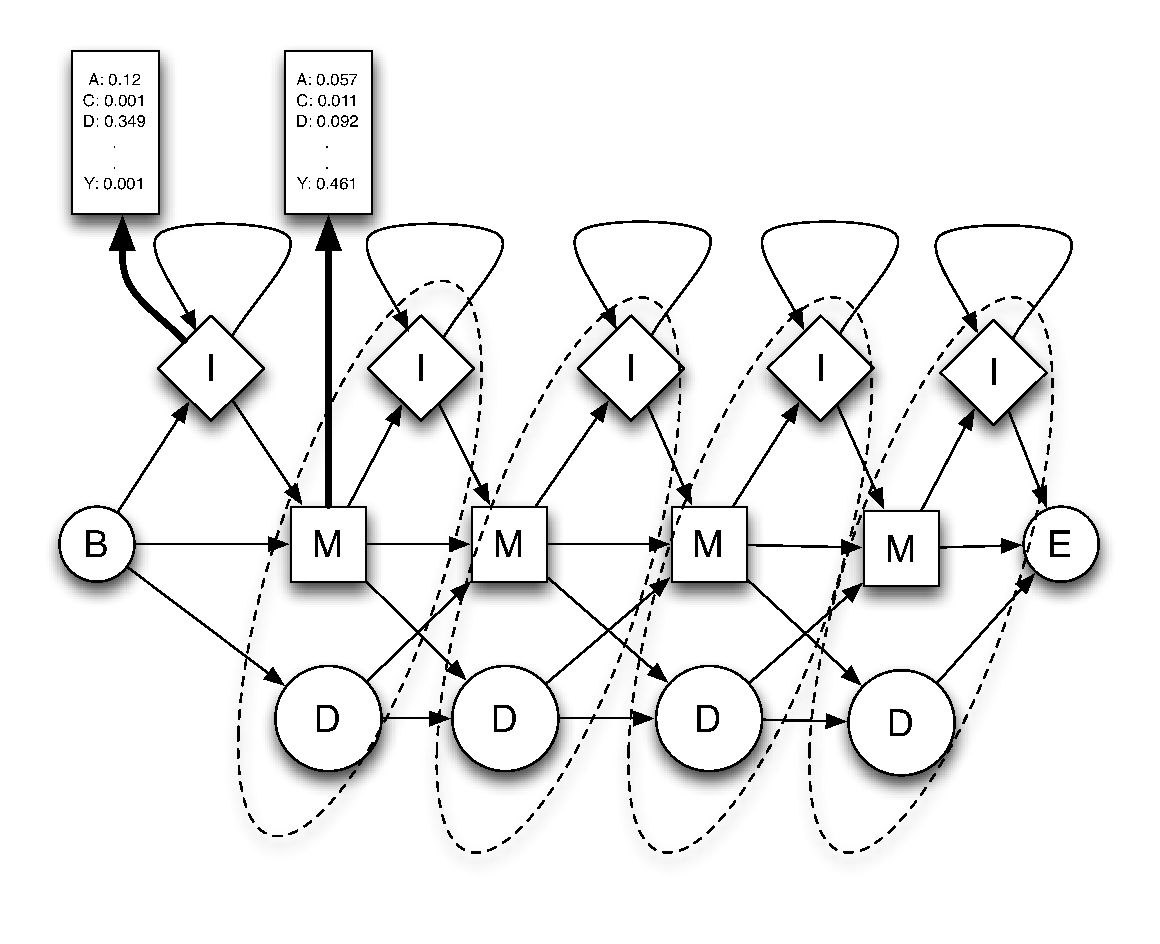
\includegraphics[width=8cm]{Plan7.eps}} 
\fi


This model
has begin and end states $B$~and~$E$,
as well as four
nodes, each containing 
an insertion state~$I$, 
a match state~$M$, and a
deletion state~$D$.

\caption{A hidden Markov model $(\alignwidth = 4)$}

\label{plan7} \end{figure}



\begin{figure*}
\newcommand\vsum[2]{#2&{}+{}& #1}

\def\goo{18pt}
\def\gum{14pt}
\[
\begin{array}{l@{}c@{}l}
V_{j}^{M}(i) &{}={}& \log\frac{e_{M_{j}}(x_{i})}{q_{x_{i}}} + \max \left\{
\begin{array}{l@{}c@{}l}
\vsum{V_{j-1}^{M}(i - 1)} {\log a_{M_{j-1}M_{j}}}\\
\vsum{V_{j-1}^{I}(i - 1)} {\log a_{I_{j-1}M_{j}}}\\
\vsum{V_{j-1}^{D}(i - 1)} {\log a_{D_{j-1}M_{j}}}\\
\end{array} \right.\\[\goo]
V_{j}^{I}(i) &=& \log\frac{e_{I_{j}}(x_{i})}{q_{x_{i}}} + \max \left\{
\begin{array}{l@{}c@{}l}
\vsum{V_{j}^{M}(i - 1)} {\log a_{M_{j}I_{j}}}\\
\vsum{V_{j}^{I}(i - 1)} {\log a_{I_{j}I_{j}}}\\
\end{array} \right.\\[\gum]
V_{j}^{D}(i) &=& \max \left\{
\begin{array}{l@{}c@{}l}
\vsum{V_{j-1}^{M}(i)} {\log a_{M_{j-1}D_{j}}}\\
\vsum{V_{j-1}^{D}(i)} {\log a_{D_{j-1}D_{j}}}\\
\end{array} \right.\\
\end{array}
\qquad
\begin{array}{l@{}c@{}l}
V_{j}^{\prime M}(i) &{}={}& e^{\prime}_{M_{j}}(x_{i}) + \min \left\{
\begin{array}{l@{}c@{}l}
\vsum{V_{j-1}^{\prime M}(i - 1)} {a^{\prime}_{M_{j-1}M_{j}}}\\
\vsum{V_{j-1}^{\prime I}(i - 1)} {a^{\prime}_{I_{j-1}M_{j}}}\\
\vsum{V_{j-1}^{\prime D}(i - 1)} {a^{\prime}_{D_{j-1}M_{j}}}\\
\end{array} \right.\\[\goo]
V_{j}^{\prime I}(i) &=& e^{\prime}_{I_{j}}(x_{i}) + \min \left\{
\begin{array}{l@{}c@{}l}
\vsum{V_{j}^{\prime M}(i - 1)} {a^{\prime}_{M_{j}I_{j}}}\\
\vsum{V_{j}^{\prime I}(i - 1)} {a^{\prime}_{I_{j}I_{j}}}\\
\end{array} \right.\\[\gum]
V_{j}^{\prime D}(i) &=& \min \left\{
\begin{array}{l@{}c@{}l}
\vsum{V_{j-1}^{\prime M}(i)} {a^{\prime}_{M_{j-1}D_{j}}}\\
\vsum{V_{j-1}^{\prime D}(i)} {a^{\prime}_{D_{j-1}D_{j}}}\\
\end{array} \right.\\[\gum]
\multicolumn3{l}{%
a'_{s \hat{s}} = - \log a_{s \hat{s}} 
\qquad
e^{\prime}_{s}(x) = - \log\frac{e_{s}(x)}{q_{x}}
\qquad
V_j^{\prime M}(i) = - V_j^{M}(i)
}
\\
\end{array}
\]

\caption{Viterbi's equations, in original and negated forms}
\label{viterbi}
\end{figure*}



\subsection{Computing probabilities using perspicuous Haskell}

\seclabel{viterbi}


Given a hidden Markov model, 
an~established software package called HMMER (pronounced ``hammer'') 
can compute the probability
that a new protein shares structure 
\ifnotcutting and evolutionary history \fi
with the proteins used to train the model.
The computation finds the most likely path through the hidden Markov model.
To~make best use of floating-point arithmetic, the software computes
the \emph{logarithm} of the probability of each path, by summing
the logs of the 
probabilities on the states and edges of the path \cite{Viterbi:1967hq}.
The~path that maximizes the
log of the probability is the most likely path.

The computation is specified on the left-hand side of \figref{viterbi}.
A~probability $V_j^M(i)$ represents the probability of the most
likely path of the first~$i$ amino acids in the query sequence,
terminating with placement of amino acid $x_i$ in state~$M_j$.
Probabilities $V_j^D(i)$ and $V_j^D(i)$ are similar.
These
equations are very clearly explained by
\citet[Chapter~5]{Durbin:1998wz}


To~be able to use Haskell, we had to reimplement the standard
algorithm for solving Viterbi's equations.
Haskell made it possible for us to write code that looks like the
math,
which made the code easy to write and gives us confidence that it is
correct.

Our code represents a query sequence as an immutable vector of amino
acids.
In~idiomatic Haskell, 
we might represent an individual amino acid~$x_i$
using a value of algebraic data type:
\begin{smallverbatim}
data Amino = Ala | Cys | Asp | Glu | Gly | ...
\end{smallverbatim}
But our models use a
legacy file format that represents each amino acid as a small integer.
Our representation is therefore
\smallverbatiminput{aa}
The log of a probability is a negative number.
To~make these numbers more pleasant to read, we negate them,
which eliminates hordes of minus signs from our file formats.
The negated logarithm of a probability is called a \emph{score}.
\smallverbatiminput{score}
Type \texttt{Score} has a limited \texttt{Num} instance which permits
scores to be added and subtracted but not multiplied.

In a hidden Markov model, each transition is actually labeled with a
score, not a probability.
And we include the labels of the states that are
connected:\remark{\emph{Why} are the labels there?
And since they are apparently never used, why do they have strictness annotations???}
\smallverbatiminput{tprob}
In~a Plan7 hidden Markov model, as discussed above, 
there are seven transitions into each node:
\smallverbatiminput{tprobs}
In~our code, we select from this 7-tuple using the \texttt{ascore}
function:\remark{Norman: please put ascore into a file}
%\smallverbatiminput{ascore}
In MRFy, the first two arguments to \texttt{ascore} are known at compile
time, and we expect \texttt{ascore} to be inlined.

Nodes are numbered, and the representation of a node includes 
the tables
of emission probabilities for the match and insertion states,
plus
the
probabilities of transitions 
into the states of that node.
\smallverbatiminput{hmmnode}

In~Viterbi's equations,
the probability in each state is a function of the probabilities
in its predecessor states, 
and all probabilities can be computed by a classic dynamic-programming
algorithm.
This algorithm starts at the begin state,
computes probabilites in nodes $1$~through~$\alignwidth$ in
succession, and terminates at the end state.
One of us implemented this algorithm, storing the probabilities in an array.
The cost was
$O(|N|\times|\alignwidth|)$;
in~MRFy, $\alignwidth$~and~$N$ range from several hundred to a few
thousand.



%%  For 
%%  reasons including floating point underflow, the HMMER software (with which we 
%%  maintain file format compatibility) stores all probabilities in a trained HMM 
%%  file as negative natural logs.
%%  Thus, the Viterbi recurrence relations are 
%%  simplified from the form in \ref{viterbi_eqn} to that in \ref{viterbi_log_eqn}, 
%%  and because they are \textit{negative} logs, the problem transforms from 
%%  maximization to minimization.

Another of us was curious to try coding Viterbi's equations
directly as recursive functions.
Like the classic recursive Fibonacci function, Viterbi's functions,
when implemented \naive ly,
perform extraordinarily badly.
But just like the Fibonacci function, Viterbi's functions can be
\emph{memoized}.
Our code implements a transformed version of Viterbi's equations, 
which operates on scores instead of on probabilities.
This version is
shown on the right-hand side of \figref{viterbi}.
The transformed equations minimize the
score (i.e., the negated log probability) for each combination of
node~$j$, amino 
acid~$x_i$, and state $M_j$, $I_j$, or $D_j$.

Scores can be usefully paired with many types of values,
so we have defined a small abstraction:
\smallverbatiminput{vscore}
Think of a value of type \texttt{Scored~a} as a container holding
 an~``\texttt a'' with a score written on the side.
The \texttt{/+/} function adds to the score without touching the
 container.

We~also made \texttt{Scored} an instance of~\texttt{Ord}.
Containers are ordered by score alone, so applying
\texttt{minimum} to a list of scored things chooses the thing with the
smallest (and therefore best) score.



The \texttt{Scored} abstraction makes it easy to implement
Viterbi's equations.
For example, to compute $V_j^{\prime M}(i)$ using the equation at the top
right of \figref{viterbi}, we call 
\mbox{\texttt{vee\char`\'} \texttt{Mat} $j$ $i$}, 
which chooses the best (\texttt{minimum}) solution
from among the three predecessor states:
\smallverbatiminput{vfix}

In this code, we look up emission scores for a given node and amino
acid using \texttt{eScore},
we~use~\texttt{/+/} to add transition and emission scores,
and we use \texttt{extend} to add \texttt{Mat} to the list of states
encountered up to this point.

Function~\verb+vee''+ is the \emph{memoized} version of~\verb+vee'+.
Calling~\verb+vee''+ produces the same result as calling~\verb+vee'+,
but faster: 
\smallverbatiminput{memo}
Functions \texttt{Memo.memo3} and \texttt{Memo.arrayRange} come from
Luke Palmer's
\path{Data.MemoCombinators} package.
The value
\texttt{numNodes} represents~$\alignwidth$,
and \texttt{seqlen} represents~$N$.

Memoization makes \verb+vee'+ perform just as well as the classic
dynamic-programming code.
And~the call to \texttt{Memo.memo3} is the \emph{only} part of the code
devoted to dynamic programming.
By~contrast, standard implementations of the Viterbi algorithm, such as in HMMER,
spend much of their code 
managing dynamic-programming tables.
Haskell enabled us write simple, performant code with little effort.
%
Because the memoized version so faithfully resembles the equations in
\figref{viterbi}, we~retired the classic dynamic-programming version.



%%  
%%  
%%  In this, we were grateful for the resemblance 
%%  between the mathematical description of the algorithm and the top-down 
%%  dynamic-programming approach in Haskell, which resulted in perspicuous code.
%%  
%%  


\subsection{Exploring new algorithms using higher-order functions}

\seclabel{hofs}
\seclabel{mrfy}

Our Haskell code for hidden Markov models and Viterbi's algorithm
solves the same problems as existing C++~code.
Other researchers using Haskell may also have to reimplement code,
but researchers may also reimplement code out of choice, not
necessity.
For~example, both SMURF and HMMER contain new implementations of these
same algorithms.
In~MRFy, we are using the Haskell implementations to help solve new
problems. 

When a real protein folds in three dimensions, 
amino acids 
that are far away in the one-dimensional sequence can be
adjacent in three-dimensional space.
We~are studying groups of such acids called \emph{beta
strands}.\remark{Fix this; we're not really studying beta strands}
Beta strands
can become hydrogen-bonded to each other,
making them ``stuck together.''
MRFy detects homologous proteins that include hydrogen-bonded beta
strands; using prior methods, many instances of this problem are
intractable. 

To~account for beta strands, computational biologists must use both a
richer model of protein structure and a revised version of Viterbi's
equations.
The~richer model recognizes that only certain pairs of amino acids are
able to bond to each other.
%%  The presence of beta strands changes both the natu
%%   the probability that a given
%%  query sequence fit
%%  A~mutation in a paired beta strand may break the pairing, in which
%%   case the mutated protein will not fold properly and is unlikely to
%%   survive natural selection.
%%  But a mutation in a paired beta strand \emph{can} survive if it is
%%   accompanied by a \emph{compensatory} mutation in the strand with which it is
%%   paired. 
When column~$j$ of an alignment is part of a beta strand and is paired
with another column  $\pairedwith j$,
the probability of finding amino acid~$x_i$ in column~$j$ 
depends on~$x_{\pairedwith j}$.
The~relevant term in
Viterbi's equations 
$V_{j}^{\prime M}(i)$ becomes
$$W_{j}^{M}(i) = V_{j}^{\prime M}(i) - \log P(x_{i} \mid x_{\pairedwith j}).$$
Columns~$j$ and $\pairedwith j$ can be as close together as a few
columns or as far apart as a few hundreds of columns.
Because $W_j^M(i)$~depends not only on $x_i$ and its local neighbors but
also on the nonlocal $x_{\pairedwith j}$, 
dynamic programming cannot compute the maximum likelihood quickly
\cite{Menke:2010ti,Daniels:2012}.
MRFy explores new methods of \emph{approximating}
maximum likelihood.

The presence of beta strands also changes the model.
Within a beta strand, amino acids are not inserted or deleted;
a~bonded pair of beta strands is modeled by
 a pair of sequences of match states.
Between the beta strands, the model is structured as before.
The~combined model, an~example of which is shown in \figref{mrf}, is called a
\textit{Markov random field}. 




MRFy treats the beta 
strands in the model
 as ``beads'' which can be slid along the query sequence.
A~positioning of the beta strands is called
 a \emph{placement}.
A~placement's probability is computed
based on observed frequencies of paired amino acids in 
hydrogen-bonded beta strands~\cite{Cowen:2002p588}.
Given a placement, the maximum likelihood of the remaining parts of
the query sequence, which appear between and around beta strands,
can be computed quickly and exactly 
using Viterbi's algorithm.
The exact result is a probability that is
\emph{conditioned} on the placement.

MRFy searches for placements stochastically,
trying to minimize scores.
We~are exploring several stochastic algorithms: random-mutation hill
climbing, simulated  
annealing, multistart simulated annealing, and a genetic algorithm.
Our~exploration exploits higher-order functions, existentially
quantified types, and (to a degree) lazy evaluation.



\begin{figure}
\ifpdfmadness
\centerline{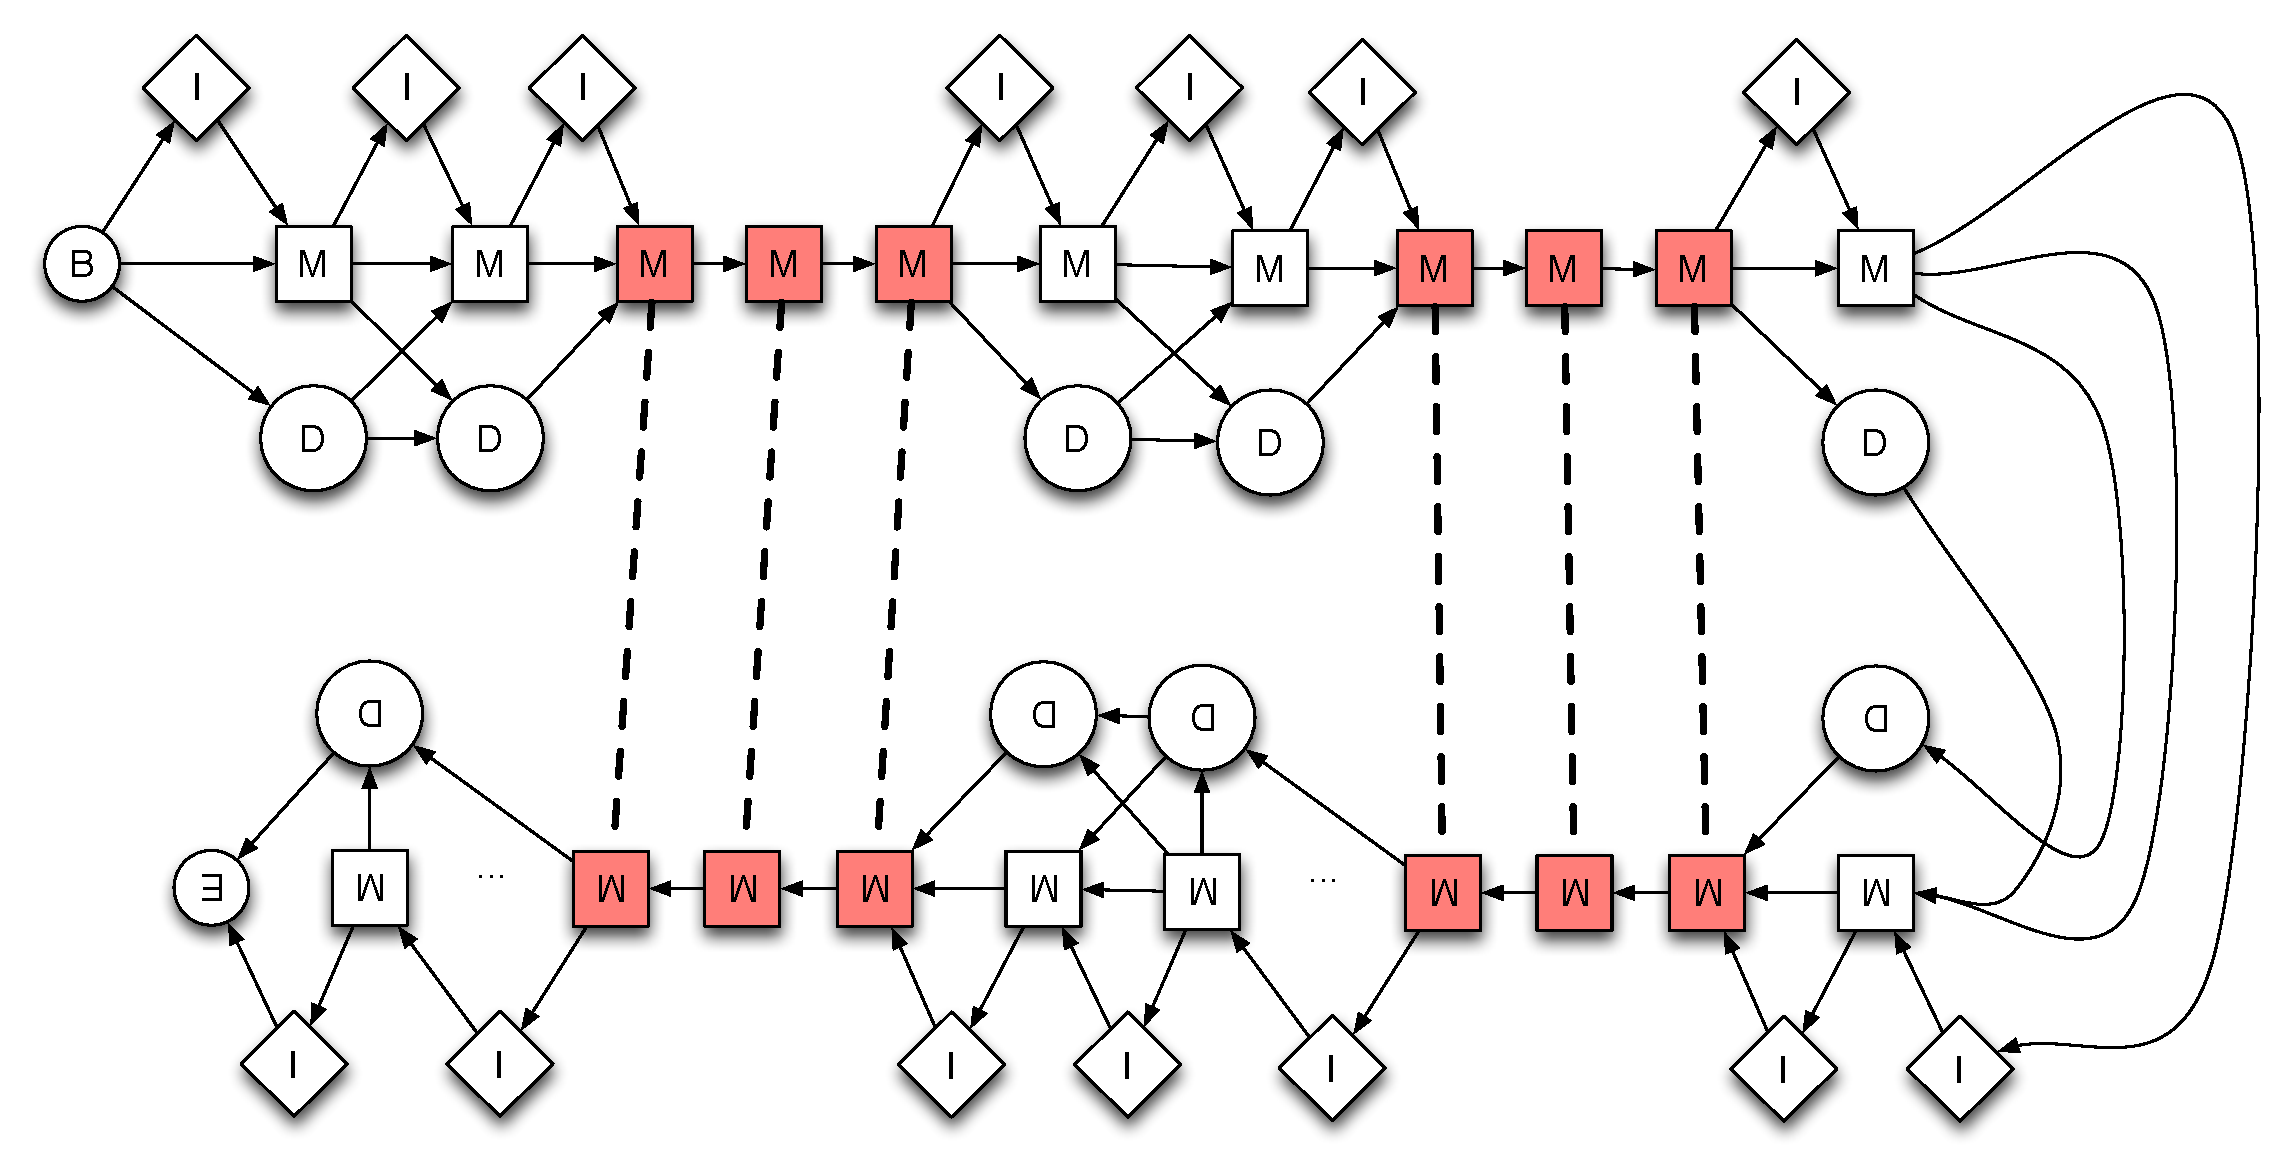
\includegraphics[width=8cm]{mrf_interleave_diagram.pdf}} 
\else
\centerline{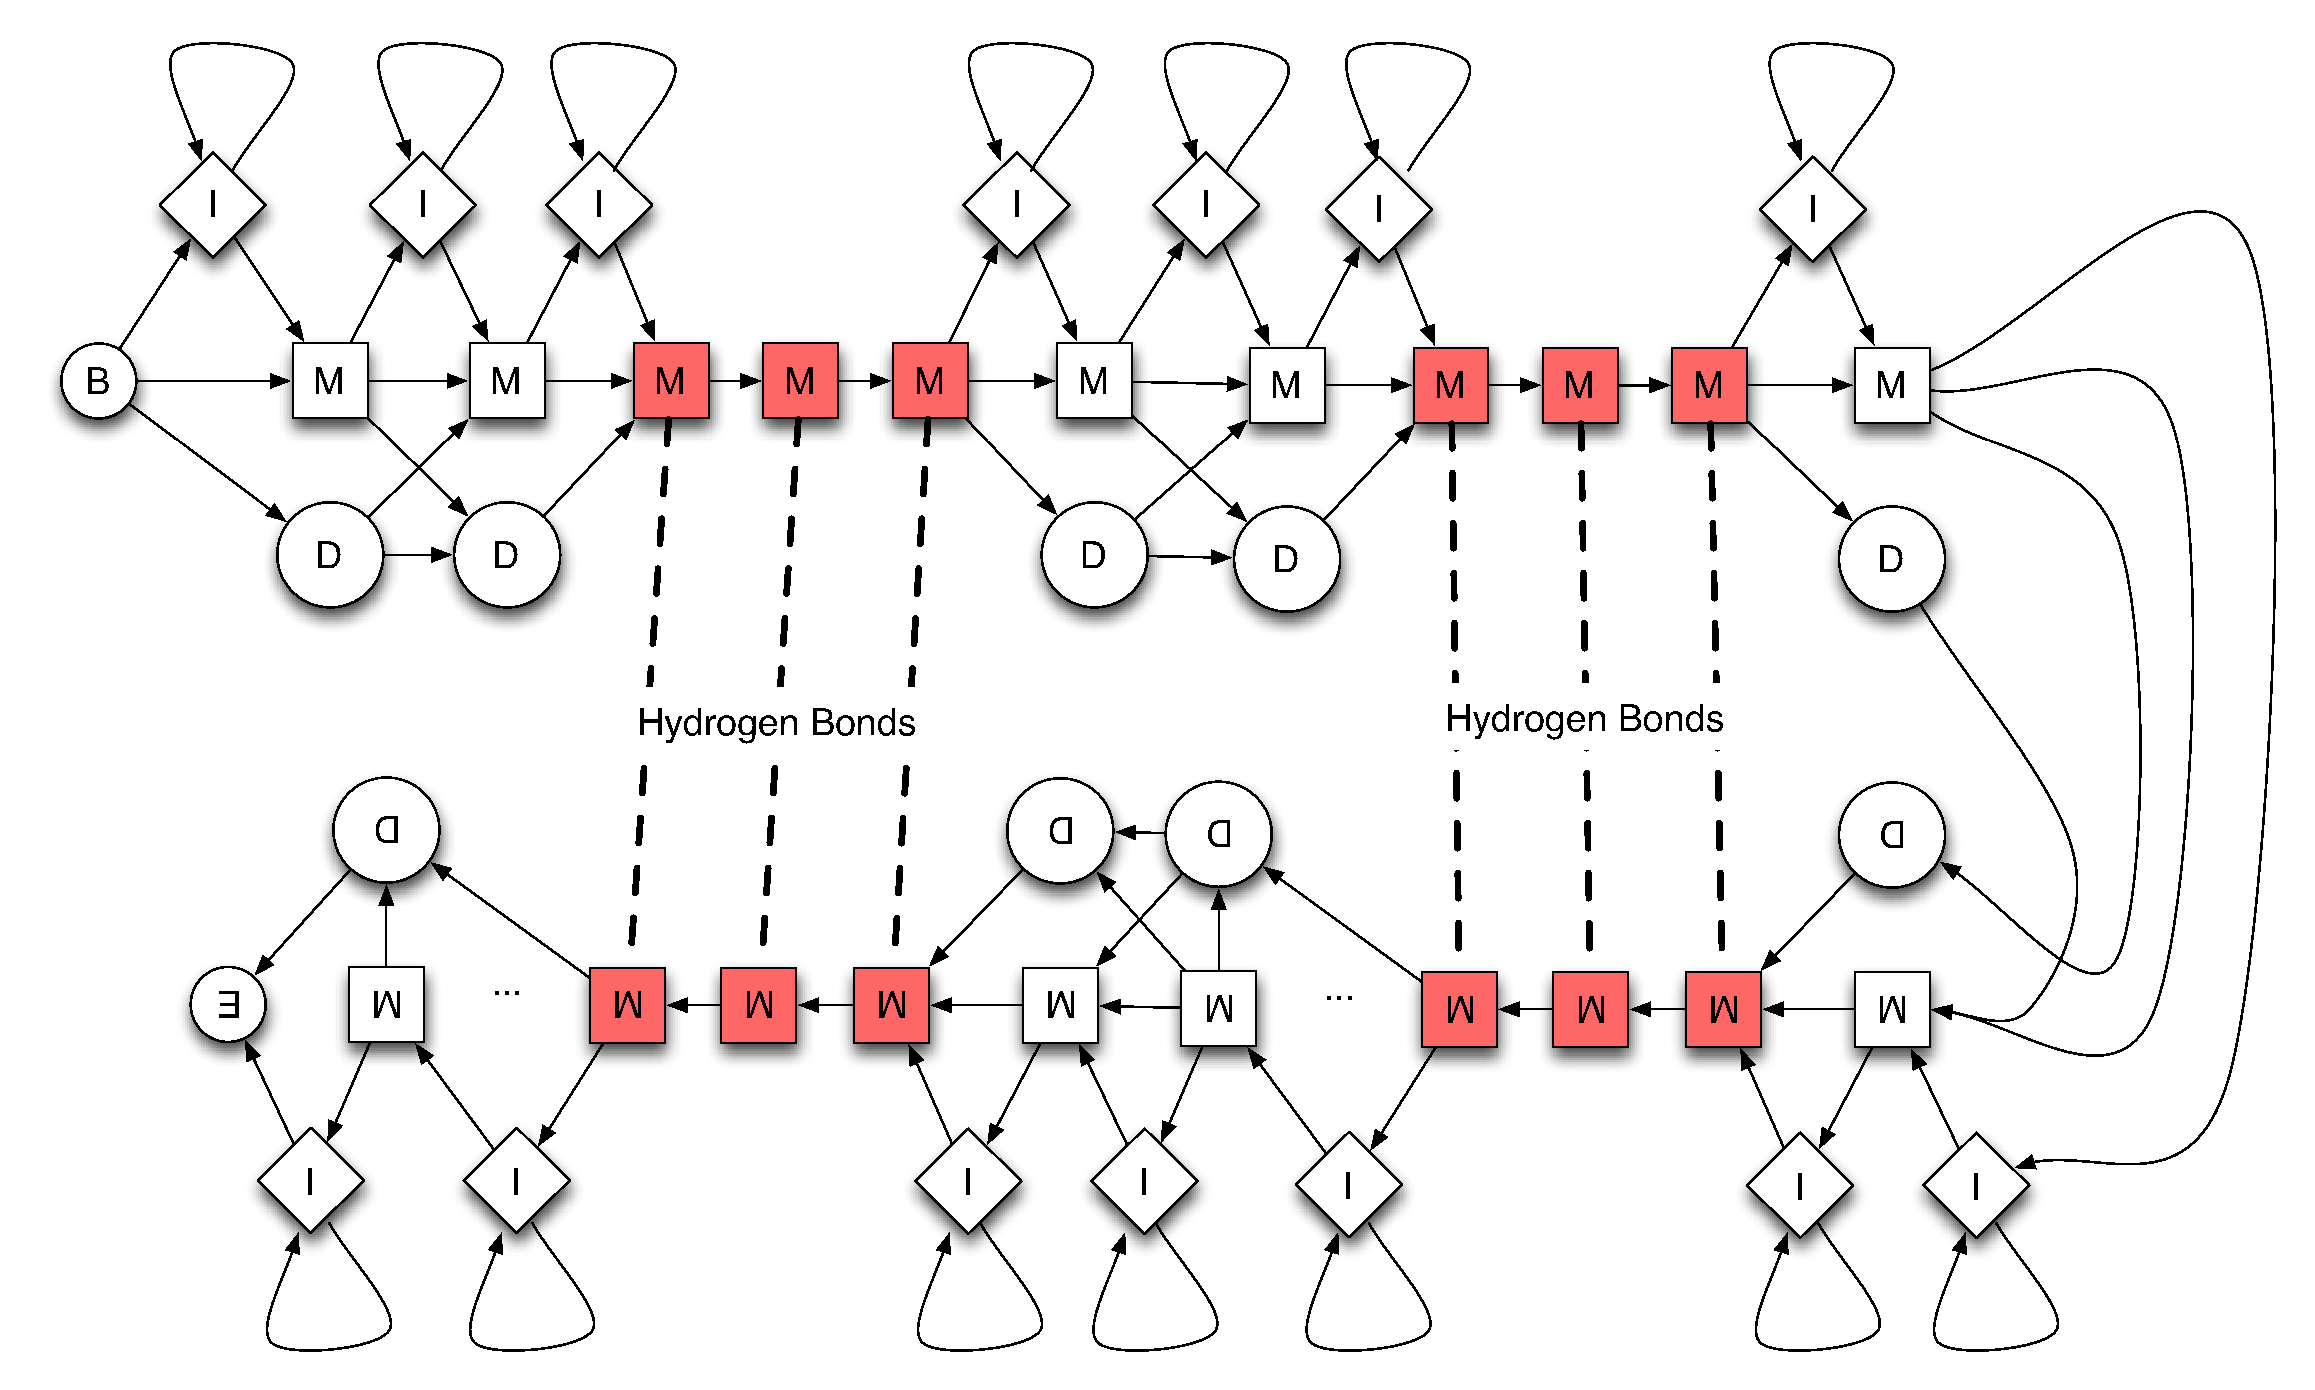
\includegraphics[width=8cm]{mrf_interleave_diagram.eps}} 
\fi
In this Markov random field,
each shaded node represents a beta-strand position.
Nodes connected by dashed edges are hydrogen-bonded.

\caption{A Markov random field with two beta-strand pairs}
\label{mrf} 
\end{figure}





We~describe \mrfy's search abstractly: \mrfy\ computes a sequence
of \emph{points}. 
Each point contains
a collection of {placements}; different searches represent
collections differently.
Each point also has a \texttt{Score}; \mrfy\ looks for points with
good scores.

Ideally, MRFy's search would use now-classic lazy, modular
technique advocated by \citet{hughes:why}, in which one function
computes an infinite sequence of points, and another function
uses a finite prefix to decide on an approximation.
But because MRFy's search is stochastic, 
making MRFy's search lazy and modular is not so easy.

To illustrate the difficulties, we~use our simplest search:
random hill climbing.
The space of beta-strand placements has no notion of slope or
gradient,
so at any given point in the search space, this search moves a random
distance in a random 
direction.
If~it leads to a better point, the move
is \emph{useful};
otherwise it is \emph{useless}.
\smallverbatiminput{utility}
(We~also use \texttt{Useful} and \texttt{Useless} to tag \emph{points}.)
With luck, an~infinite sequence of useful moves converges
at a local optimum.

\mrfy's search path follows only useful moves;
if a move proves useless, 
\mrfy\ abandons it and tries again (with a new random seed) at the
previous point.
Ideally, \mrfy\ would search by composing a \emph{generator}
that produces an infinite sequence of moves, 
a \emph{filter} that selects the useful moves, and 
a \emph{test} function that enumerates finitely many useful moves
and returns the final destination.
But the generator may produce an infinite sequence of useless moves.
(For example, if \mrfy\ should find a global optimum, every move from
that point is guaranteed to be useless.)
Given an infinite sequence of useless inputs, a filter would not be
productive, and a test function would diverge.

We~address this problem by combining ``generate and filter'' into a
single abstraction, which has type \texttt{SearchGen pt r}.
Type variable~\texttt{pt} is a point in the search
space, and type variable~\texttt{r} is a
random-number generator:
\smallverbatiminput{gen.tex}
The monadic computation \texttt{pt0} randomly selects a starting point
for search;
\texttt{nextPt} produces a new point from
an existing point.
Because scoring may be expensive, both \texttt{pt0}
and \texttt{nextPt} use \emph{scored} points, and they can
reuse scores from previous points.

Why do we have \texttt{pt0} and \texttt{nextPt}
instead 
of a single function with type \mbox{\texttt{Rand r [Scored pt]}},
which could produce an infinite list?
Because after the first move
the starting point for the next move depends on whether the first move
was useful, whereas the first move is always useful.
That decision is made by the \texttt{utility} function,
which scrutinizes a move represented as follows:
\smallverbatiminput{move}
The decision about utility uses not only a source of randomness but
also the \emph{age} of the search, which corresponds to the
computational cost to reach a point in the search.
For example, in~simulated annealing, as the search progresses,
the \texttt{utility} function becomes less likely to express a move
that results in a worse score.

\noindent
\vbox{
Using these pieces, function \texttt{everyGen} produces an infinite
sequence containing a mix of useful and useless moves:
\smallverbatiminput{everygen}
}
\noindent
Because both \texttt{nextPt} and \texttt{utility} consume randomness,
the computation is very sequential, but it does use a little bit of
laziness:
from its starting point, \texttt{everyPt} provides an infinite list of
randomly chosen successor points, then calls \texttt{agedUtility} to
tag each one with the search's age and the point's utility.
The Prelude function \texttt{span} finds the first useful successor,
but in case there \emph{is} no successor, the code must also produce
all the useless successors.
If~we do find a useful successor, we start searching anew from that
point, with a recursive call to \texttt{everyPt}.

The most telling line of code in \texttt{everyPt} is the last line of
the body, which shows that the result begins with a useful point,
is followed by a (possibly infinite, possibly empty) list of useless
points, and then continues recursively with another useful point.
When the computation returned by \texttt{everyPt} is evaluated against
a random-number generator, it returns an infinite list containing a
mix of useful and useless points.
This mix can be passed to a test function of type \texttt{SearchStop~pt}:\\
\vbox{
\smallverbatiminput{strat}
\smallverbatiminputx{stop}
\smallverbatiminputx{search}
}
\noindent


We have two kinds of non-modularity.
First, termination has to
look at \emph{all} states, even though we would prefer that it look
only at useful states.
This is because otherwise we risk non-termination:
we are not guaranteed a useful move after any finite number of steps.
Second, age of the search shows up in multiple places.
In particular, we cannot separate the age of the search at the
current state from the utility decision.

The \texttt{SearchStrategy} interface provides ample scope for
experiments.\remark{\P\ needs rewriting}
Random-mutation hill climbing took fifty lines of code and one~day to
implement.
Simulated annealing reuses hill climbing's
 \texttt{nextPt}, \texttt{pt0}, and \texttt{quit} functions.
Simulated annealing's  new \texttt{accept} function took ten
lines of code and half an hour to implement.
(Hill climbing accepts a point if and only if it scores better than its
predecessor;
simulated annealing may accept a point that scores worse.)
Our genetic algorithm reuses the same
\texttt{pt0} and \texttt{quit} functions, and its \texttt{accept}
function took only a few lines of code.
But~the recombination of parent
placements in its \texttt{nextPt} function took forty lines of code
and a full day to implement.
\ifnotcutting
Our~current \texttt{quit} function simply runs for a fixed number of
generations, but its interface will enable us to try other criteria,
such as stopping once $k$~generations have passed without more than $E$
improvement in score. 
\fi

Our \texttt{SearchStrategy} interface somewhat resembles an object-oriented
style of programming.
However, it is \textit{easier} to create a SearchStrategy
in Haskell than using conventional object-oriented techniques, because
all the functions in a SearchStrategy are partial applications of
other functions.
If we were using conventional object-oriented
techniques, we would have to declare subclasses with instance
variables and would have to write code to initialize objects of those
subclasses. 


\subsection{Performance}

\seclabel{perf}

MRFy calls \verb+vee'+ several
 times
for each placement in each search generation.
Calls on query sequences between beta strands are independent,
as are calls on different placements.
We~found them easy to parallelize
using
\texttt{Control.Parallel}:
we substituted
\texttt{parmap rseq} for \texttt{map}.
Even when there is just one placement per generation,
MRFy can keep six cores busy.
Given multiple placements per generation,
it~can use forty-eight cores.
However, we have found that MRFy performs best, at least on our
hardware, with between 12 and 16 cores.
We have access to only
one 48-core system, and while MRFy will keep all 48 cores busy, it
performs only slightly better, at an average of 35 seconds to find an alignment
on a large protein structure, than when given 16 cores, which takes an average
of 37 seconds. 

MRFy's predecessor, SMURF, does not perform stochastic search,
and thus its overall run-time performance cannot be compared directly to MRFy.
However, both programs implement the Viterbi algorithm.
On an exceedingly large, contrived example, comprising 56,000 amino acids
(larger than any known protein) and 343 nodes, and ignoring all beta-strand
information, SMURF's Viterbi implementation completed in 0.497 seconds on a
2.6GHz Core i7.
On the same benchmark, MRFy's Viterbi implementation required 1 minute 57
seconds.
Despite the inferior runtime performance, MRFy still meets our performance
goals.
This is because the stochastic search algorithm relies on the Viterbi algorithm
applied to many, significantly smaller hidden Markov models than SMURF's
multidimensional programming must tackle.
MRFy computes an alignment for a 12-stranded ``beta sandwich'' structure in
generally less than one minute, while SMURF consumes over 16GB of memory
and does not terminate even after eight hours.
Had we implemented the SMURF algorithm in Haskell, we believe that performance
would be unacceptable.
However, for the algorithm underlying MRFy, we are satisfied with the runtime
performance of Haskell and GHC.
Nonetheless, we expect that we can still improve MRFy's run-time performance
with further profiling and tuning.




In~\secref{viterbi} above, the example case for the \verb+vee'+
function computes not just a score but also an optimal path.
MRFy's \texttt{search} function, in \secref{mrfy}, uses only the
score.
Even though Haskell evaluation is lazy, the \verb+vee'+ 
still allocates thunks that could compute paths.
We~cloned \verb+vee'+ and modified it to compute
only a score, with no path, and this change improved 
run-time performance by nearly~50\%.
But when \texttt{search} finally decides on a placement, we need a
version of \verb+vee'+ that \emph{does} compute a path, so we can
extract the optimal parse for that placement.

How could we keep the performance improvement without having to
maintain two versions of \verb+vee'+?
In~Lisp or Ruby we would have used macros or metaprogramming,
but we were not confident of our ability to metaprogram a solution
using Template Haskell.
Instead, we replaced the primitive cons in \verb+vee'+ with a
call to a function of the same type, which we passed~in.
Passing the primitive~``\texttt{:}'' gives us a path,
and passing \verb+\_ _ -> []+ gives us the same
speedup as the cloned and modified~code.
But~although
this trick is simple and easy to implement, 
we~have an uneasy feeling that it may work only because of undocumented
properties of GHC's inliner, which may be subject to change without
notice. 

\subsection{Awkward Haskell}

\seclabel{awkward-profiling}

We~think \verb+vee'+ is beautiful, but we wrote some ugly code, too,
because we lack skills and knowledge in two areas.
The first is profiling.
GHC's profiling is based on cost centers \cite{sansom-pj},
and for most of MRFy's development, we used GHC 7.0, which
will happily add cost centers to top-level 
functions only, while much of our code is in nested functions.
We~know of no better technique than to add cost-center annotations to
each guard clause and nested function,
but these annotations made our code so ugly that we felt compelled to
remove them as soon as possible.
And without the annotations, GHC's call-site and allocation
profiles did not give us enough information to be useful.
We~miss valgrind, whose callgrind profiler gives useful information
without \emph{any} annotations in the source.
Late in MRFy's development, we began using GHC 7.4, which provides much
better profiling tools.
We are thrilled by these tool developments.

Our other ugly code came from  attempts to debug
run-time errors.
Our~group's legacy file
format is poorly documented: when beta
strands overlap and are doubly paired, the invariants of the
representation are not clear.
These files are hard to deal with no matter what
programming language is used, and faults are to be expected.
But using Haskell, we had a hard time diagnosing run-time errors.
Calls to
\texttt{trace} 
littered our code,
even when relegated to wrapper functions.
We~weren't aware of the backtrace feature of GHC's profiler,
and even after we discovered that feature, the results weren't good enough:
the profiler can be used only on very small test cases that didn't always trigger
run-time errors.
This same limitation affected the GHCi debugger; our \texttt{vee'} function
shown in \secref{viterbi}, when it is not compiled with
optimizations, requires too much run time to be practical on non-trivial
inputs.
Moreover, the GHCi debugger can only set breakpoints at top-level functions
or at specific column/line positions, which made debugging the memoized
\texttt{vee''} function impractical.
In~August 2011, 
Lennart Augustsson said that the biggest advantage of Strict
Haskell is getting a stack trace on error,
and Simon Marlow said that he may have figured out how to track call
stacks properly in a lazy functional language.
We~can't wait.

\remark{The following \P\ will need to be connected up to the last \S\
on ``our old approach to debugging.''}

Debugging led also not to awkward code, but to awkward interactions on
our team.
The two junior members of the team wanted to apply the debugging
skills they had honed through years of imperative programming.
The senior partner kept nattering on about QuickCheck properties.
No~progress was made until the first draft of this paper was prepared.
At~that point, we were quickly about to write QuickCheck
specifications for several properties of the Viterbi algorithm:
\begin{itemize}
\item
The total number of \verb+Mat+ and \verb+Ins+ states returned equals
the number of amino acids in the query sequence.
\item
The total number of matches, and deletions returned equals the
number of nodes in the hidden Markov model,
\emph{except} that an initial sequence of
of~\verb+Ins+ states counts as a single node,
due to an odd property of the HMMER file format (namely, the zeroth
node has no delete state and a non-emitting match state which
is always occupied, but a normal insert state).
\item
The sequence returned satisfies the Plan7 invariant, that is, states
\verb+Ins+ and \verb+Del+ are never adjacent.
\end{itemize}
\textbf{These properties need to be followed by more ambitious
properties},
such as proving that nearby sequences are less likely than the
sequence returned by \verb+vee'+.
One practice we recommend for those following in our footsteps is to
write instances of \texttt{Arbitrary} for data types as those data types
are written, when relevant invariants are fresh in memory.

This was a practice that the junior members of our team did not follow, and
they sorely regret it.
We speculate that one reason why we didn't follow this practice was a poor 
understanding of the \texttt{Arbitrary} type class.
Namely, a lot of the examples we had seen using QuickCheck focused 
predominantly on writing and testing properties with data types that already 
implemented \texttt{Arbitrary}.
We recall a smattering about \texttt{Arbitrary}, but we were still too baffled 
by the \texttt{Gen} monad to truly grasp its importance in using QuickCheck.
When it finally came time to use QuickCheck, we were overwhelmed by the amount 
of work that had to be done to write and test implementations of 
\texttt{Arbitrary} for each of our data types.


 
 
\section{Our previous experience compared}
\seclabel{comparo}

When performance has mattered, members of our group, like other
computational biologists, have used~C++.
We~compare our experience with three tools:
\begin{itemize}
\item
Matt~\cite{Menke:2008wu} is used to create alignments like that shown
in \figref{alignment}.
It~comprises about 12,000 lines of~C++.
The only external tools or libraries it uses are \texttt{zlib}
and \texttt{OpenMP}, and its initial development took two years.
\item
SMURF
\cite{Menke:2010ti} is used to detect homologous proteins in the presence
of paired beta strands.
It~comprises about 9,000 lines of~C++, of which about 1,000~lines are
shared with~Matt.
It~uses no external tools or libraries, and
its initial development took a year and a half.
It uses multidimensional dynamic programming to exactly compute the alignments
for which MRFy relies on stochastic search.
As a result, in the presence of complex beta-strand topologies, SMURF is
computationally intractable.
\item
MRFy is used to detect homologous proteins in the presence of paired
beta strands; it effectively supplants SMURF.
It~comprises about 1,200 lines of~Haskell.
It~uses several external tools and libraries, of which the most
notable are Parsec, the BioHaskell bioinformatics library, and
the libraries \path{Data.MemoCombinators}, \path{Control.Parallel},
and \path{Data.Vector}.
Its initial development took about three months.
%%%% \remark{Others were mostly full-time work, but no need to distinguish.}
\end{itemize}
Like much research software, all three of these tools were written
 in~haste.
We~have experience modifying the older tools.



We~modified Matt to use information about sequences as well as structure.
The modification added 2,000 lines of code, and it calls
external sequence aligners that we did not write.
We~thought the modification would take three months, 
but it took most of a~year.
Matt uses such
data structures as mutable oct-trees, vectors, and arrays.
It~uses clever pointer arithmetic.
The mutable data structures were difficult to 
repurpose, and the pointer arithmetic was \emph{too} clever: 
nearly every change resulted in new segfaults.

We~had hoped to extend Matt further, with support for partial alignments,
which we~expected to require only 
a cosmetic manipulation of the 
output.
But
this feature wound up
requiring deep information about Matt's data structures,
and we had to give~up.
We~believe we could write an equivalent tool in~Haskell,
with most of Matt's performance, in at most nine months.

Our most painful experience was adding ``simulated evolution''
to~SMURF \cite{Daniels:2012}. 
Although simulated evolution represents a relatively minor
enhancement,
just understanding the existing code took several months.

We~built MRFy quickly, and we expect that
higher-order functions will make MRFy easy to extend.
Each new addition to MRFy's stochastic search has taken at most a day
to implement.

Haskell encourages hasty programmers to slow down.
We~have to get the types right,
which makes it hard to write very large functions.
To~get the code to typecheck, we~have to write type signatures, which
also serve as documentation.
And once the types are accepted by the compiler,
it~is not much more work to write contracts for important functions.
MRFy is still hasty work.
Many types could be simplified;
we're~sure we've missed opportunities for abstraction;
and we know that MRFy's decomposition into modules could be improved.
But despite being hasty programmers, we produced code 
that is easy to understand and easy to extend.
Our hastily written Haskell beats
our hastily written Ruby and~C++.

We~can also make a preliminary comparison of performance.
SMURF can parse a simple protein structure, optimally, in under 10~seconds.
It~can parse some more complex structures in 2--3~minutes.
But when asked to parse the most complex structures, it runs out of
memory and has to be killed, even on a system with 128GB of~RAM.
By~contrast, MRFy can parse any of these structures, approximately,
in 30~seconds.
This performance
meets our goals, and it means that MRFy can be used to scan whole genomes.




Looking beyond our research group to computational biology more
broadly, our experience with other software is better.
Little of it is written in functional languages, 
but much of the software shared by the community is excellent.
MRFy's training component was derived from that of~HMMER,
and
working with the HMMER 
codebase was pleasant;
data structures and their
mutators are well documented. 
There is a 
BioHaskell library, part of which we use,
but it is not nearly as 
complete as BioPython or BioRuby, which are heavily used in the community.
We hope that tools for computational biology in
Haskell continue to mature. 

\section{What can you learn from our experience?}

If~you are a computational biologist, 
you can be productive in Haskell, and you don't need extensive
experience.
Two~of us (Daniels and Gallant) are graduate students.
Daniels has taken a graduate seminar in functional programming, which
included some Haskell;
Gallant has taken a programming-languages course which included
significant functional programming but no Haskell.
Ramsey is a professor who has used Haskell 
for medium-sized projects,
but his contribution to MRFy was limited to minor ranting and refactoring.


\subsection{Barriers to be overcome}

In~\secref{awkward-profiling} above, we~mention the awkwardness of the
cost-center annotations required for profiling.
But~we also found it difficult just to get the profiler working.
In~particular, profiling requires that all installed libraries be recompiled
with profiling support.
We~were not able to achieve such recompilations consistently.


We~faced another barrier in testing.
One of us (Ramsey) kept ranting that we should test our code using 
QuickCheck \cite{claessen:quickcheck},
but we could never figure out~how.
We~were stumped by two problems:
how to break down MRFy into parts that could be
unit-tested,
and how to implement QuickCheck generators for representations of complex
data like beta-strand placements.
We~know that QuickCheck is a powerful and proven tool,
but we could not figure out how to exploit~it.

Like other functional programmers, we~have found that 
once we have our types right, our code is often right.
But~MRFy computes with arrays and array indices,
and in that domain, types don't help much.
Bounds violations lead to run-time errors, which we have not been able
to identify any systematic way to~debug.
GHC's profiler can provide stack traces, but we~found this information
difficult to discover, and as noted above,
there are barriers to profiling.
We're~aware that debugging lazy functional programs has been a topic
of some research,\finalremark{Do we cite Hood, Hat, or Freya?}
but one of the biggest barriers we encountered to using Haskell is
that we have had to abandon our old approaches to debugging,
and we~see no clear path to follow.


\subsection{Information that will help you succeed}

If~you want to use Haskell in your research, we~believe that you must
have enough experience with functional programming that you can build
\emph{all} the code you need, not only the code that is easy to write
in a functional language.
Implementing Viterbi's equations in Haskell was pure joy.
Writing an iterative search in purely functional style was~easy.
Transforming data in the HMMER file format, \emph{without}
using mutable state the way the C++ code does, was difficult.

\seclabel{penumbra}

You~also need to know that while the Haskell community offers many
enticing tools, libraries, and packages,
not all of them are worth using.
Some are not ready for prime time, and some were once great but are
no~longer maintained.
The great packages, like \texttt{Data.MemoCombinators} and Parallel
Strategies, are truly great.
But~for amateurs, it's not always easy to tell the great packages from the wannabes
and the has-beens.
And even some of the great packages could be better documented, with
more examples.

%%  Most of the software we used came from Hackage, which is the Haskell
%%  community's software repository.
%%  We~sometimes found it hard to tell
%%  if a particular Hackage package was right for us.
%%  In particular, as beginning 
%%  functional programmers, we~found some documentation inaccessible.
%%  The documentation that we found most accessible typically contained
%%  examples showing how to use a particular tool or library.
%%  \remark{So what's our message here? What are we telling people to
%%  think or do differently? ---NR}


As~in any endeavor, it's helpful to have access to experts.
We~would have been better off if our in-house expert had been an
enthusiastic student and not a busy professor.
But we have been surprised and pleased by the help available from
faraway experts on Stack Overflow and on Haskell mailing lists.
Although a local expert makes things easier, one is not
 absolutely necessary.

MRFy is available at \url{mrfy.cs.tufts.edu}

\section{Conclusion}

A~little knowledge of and a lot of love for functional programming
enabled us to carry out a successful research project in a language
that computational biologists seldom use.
If~you \emph{want} to use Haskell---or one of your graduate students
wants to use Haskell---you can
succeed. 




% - No obvious body of knowledge on code improvement. 
%  

 

\ifnotcutting
\acks

An~anonymous referee spurred us to think
more deeply about laziness.
Josef Svenningsson suggested a correspondence between \mrfy's search
and stream fusion, which led us eventually to the \texttt{Utility} type.
We also thank Lenore Cowen, Kathleen Fisher, Ben Hescott, Brad
Larsen, and Nathan Ricci. 
\fi


\bibliographystyle{plainnat}

% The bibliography should be embedded for final submission.

\bibliography{mrfy_experience_report}

\iffinaldraft


\vfill

\begingroup
\parfillskip=0pt
\advance\leftskip by 0pt plus 30em
\emph{You can live to surf the Haskell wave, but~if you slide off the crest, you
drown.}
\par
\endgroup

\fi

%%%%    \break
%%%%    
%%%%    
%%%%    \appendix
%%%%    
%%%%    
%%%%    \section{Orphaned text}
%%%%    
%%%%    
%%%%    In~our C++ work, the faults we encounter most frequently are
%%%%    segmentation faults, 
%%%%    memory errors caused by pointer arithmetic or uninitialized 
%%%%    memory,
%%%%    and heap exhaustion.
%%%%    In~our Haskell work, the faults we encounter most frequently are
%%%%    type errors and bounds-checking errors in array and vector accesses.
%%%%    While we have found the bounds-checking errors difficult to debug,
%%%%    they are less difficult than memory errors.
%%%%    
%%%%    
%%%%    Implementing the equation in this form was not only intellectually
%%%%    satisfying; it~also helped us find
%%%%    bugs.
%%%%    The most memorable bug was that in one of our base cases, 
%%%%    we~mistakenly returned an empty path of states;
%%%%    the correct result was a singleton path containing the initial state.
%%%%    Very quickly after observing a missing state in the output, we were
%%%%    able to find the faulty case in the code.
%%%%    
%%%%    
%%%%    

\end{document}
